\documentclass[UTF8]{book}
\usepackage[fontset=adobe]{ctex}
\usepackage{float,xcolor}
\usepackage{graphicx}
\usepackage{multicol}
\usepackage{makeidx}
\usepackage{cite}
\usepackage{wasysym}
\usepackage[colorlinks]{hyperref}

\newCJKfontfamily{\dejavusanszh}{DejaVu Sans} % this font has the required glyphs
\newfontface{\dejavusans}{DejaVu Sans} % this font has the required glyphs
\newcommand{\iching}[1]{{\dejavusanszh\char\numexpr"4DC0+#1}}
\newcommand{\trigram}[1]{{\dejavusans\char\numexpr"2630+#1}}

\setCJKmainfont[BoldFont=Adobe Heiti Std,ItalicFont=Adobe Kaiti Std]{Adobe Song Std}
\setCJKsansfont{Adobe Heiti Std}
\setCJKmonofont{Adobe Fangsong Std}
\makeindex
\begin{document}
  \title{观澜札}
  \author{半夏}
  \date{\today}
  \maketitle
  \setcounter{tocdepth}{2}
  \tableofcontents
  \part{释家}
\chapter{历史}
\section{印度佛教史}

\subsection{种性制度}
\begin{itemize}
  \item 婆羅門:祭司
  \item 剎帝利:武士
  \item 吠舍: 农工商业
  \item 首陀羅: 奴隶
\end{itemize}

\subsection{六派哲學}
產生於史詩時期之末,與佛教初期階段相近的婆羅門教哲學\footnote{木村泰賢$\cdot$《原始佛教思想論》}。
\begin{itemize}
  \item 尼夜耶派(The Nyāya School)。
  \item 僧佉耶派(The Sāṃkhya School)即數論派。
  \item 毘舍迦派(The Vaiśeṣika School)即勝論派。
  \item 瑜伽派(The Yoga School)。
  \item 弭曼差派(The Mīmāṃsā School)。
  \item 吠檀多派(The Vedānta School)。
\end{itemize}

\subsection{奧義書}
\begin{itemize}
  \item 業說,在《古奧義書》本為不公開的密教,到佛世則成為各教派所公認的思想
  \item 輪迴說,在梵書時代已萌芽,完成而為一般所承認,則自奧義書時代始
  \item 解脫說,乃為《奧義書》的最終目的
\end{itemize}

\subsection{六師外道}
記載常見於声闻經律\footnote{《長阿含經》第二十七經《沙門果經》}
\begin{itemize}
  \item 不蘭迦葉(Pūraṇa-Kāssapa):為倫理的懷疑者,否定善惡之業有其相應之根,故倡無作用論。
  \item 末伽梨瞿舍利(Makkhali Gosāla):此為邪命外道之祖,倡無因而有論。乃是耆那教的一派,在佛世極有勢力,除了耆那教,他是其餘五師中最盛大者。
  \item 阿耆多翅舍欽婆羅(Ajita Keśakambala):否定靈魂之說,倡唯物論,以快樂為人生之目的,排斥一切嚴肅的倫理觀念,此亦即是順世外道。
  \item 婆浮陀伽旃那(Pakudha Kaccāyana):主張心物永不消滅,倡世間常存論。
  \item 散若夷毘羅梨沸(Sañjaya Belaṭṭhiputta):為詭辯派或捕鰻論者,舍利弗(Śāriputra)及目犍連(Mahāmaudgalyāyana),即是此派出身而皈信佛教的。
  \item 尼乾陀若提子(Nigaṇṭha-Nātaputta):這就是耆那教之始祖摩訶毘盧(Mahā-vira),他出世稍早於釋尊,也是王子出身。此派以命(Jīva)及非命之(Ājīva)之二元論而說明一切,故也是否定有上帝造物觀念的無神論者。其實踐方面,則以極端的苦行及嚴守不殺生為特色。
\end{itemize}

\subsection{六十二見}
兩說及十類\footnote{《長阿含經》卷一四第二十一經《梵動經》}
\begin{itemize}
  \item 說過去世,或稱本劫本見者,五類十八見:
    \begin{itemize}
      \item 世間常住論,即是常見論,四種。
      \item 世間半常半無常論,四種。
      \item 世間有邊無邊論,四種。
      \item 異問異答論,即是詭辯派、捕鰻論、不死矯亂論,四種。
      \item 無因而有論,即是無因論,二種。
    \end{itemize}
  \item 說未來世,或稱末劫末見者,五類四十四見:
    \begin{itemize}
      \item 世間有想論,十六種。
      \item 世間無想論,八種。
      \item 世間非有想非無想論,八種。
      \item 眾生斷滅無餘論,即是斷見論,七種。
      \item 現法涅槃論,即無論在何種狀態,處於現世的即為最高的境界,五種。
    \end{itemize}
\end{itemize}

\subsection{家谱}
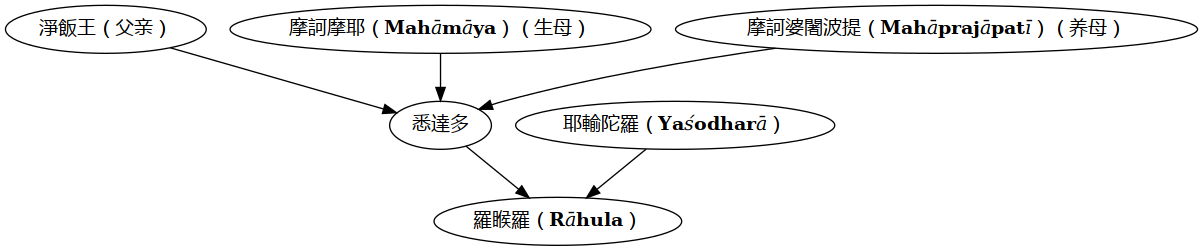
\includegraphics[width=\textwidth]{释家/images/释尊家谱.png}

\subsection{修道}
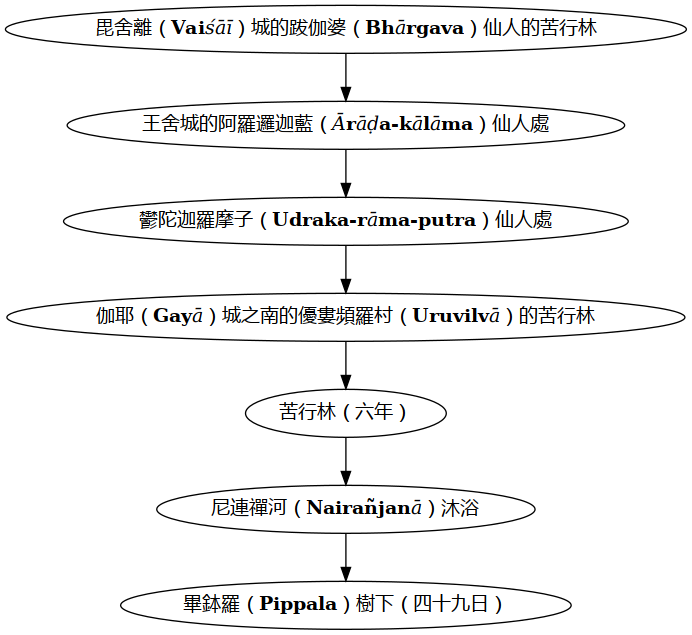
\includegraphics[width=\textwidth]{释家/images/释尊修行地图.png}

\subsection{四七日}
\begin{enumerate}
  \item 在菩提(Bodhivṛkṣa)樹下。就是那棵畢鉢羅樹之下,因佛在此樹下成道,而被稱為菩提樹
  \item 在阿踰波羅(Ajapāla)樹下。此期有魔王波旬(Māra-pāpīmān)來請佛入滅而未果。
  \item 在目真鄰陀(Mucilinda)樹下,遇暴風雨,目真鄰陀龍見之而即以己身護佛。此龍即受皈依,乃為傍生中的第一弟子。
  \item 在羅闍耶恆那(Rājāvatana)樹下。有二商主,一名提謂,一名婆梨迦,道經佛處,以麨蜜供佛,並皈依佛、法而去。此二人乃為最早的優婆塞(Upāsaka 親近而奉事三寶的淨信男)
\end{enumerate}

\subsection{轉法輪}
\begin{enumerate}
  \item 婆羅奈斯(Vārāṇiasī)城的鹿野苑度五比丘,接著又度了耶舍(Yaśa)及其親友數十人
    \footnote{ 阿若憍陳如(Ājñāta-Kauṇḍinỵa)、跋提(Bhadrika)、婆波(Vāṣpa)、摩訶男(Mahānāma)阿說示(Aśvajit)}
    \footnote{自此即有了教主、教法、教團的(佛、法、僧)三寶具足}
    \footnote{滿慈子、大迦旃延、婆毘耶等,亦捨外道法而進入佛法。}
    。
  \item 在鹿野苑度過第一個雨季的安居生活,釋尊便囑咐弟子們各各遊化人間,弘揚佛陀的教義
    \footnote{乃至要弟子們不應兩個人同走一條路};
    佛陀自己也單獨去到優婁頻羅聚落
    \footnote{化度了事火外道優婁頻羅迦葉(Uruvilvā-kāśyapa)和他的兩個弟弟那提迦葉(Nadī-kāśyapa)、伽耶迦葉(Gayā-kāśyapa),以及他們三人的弟子共一千人。}
    。
  \item 釋尊為了履行成道之後去度頻婆沙羅王的諾言,便率領迦葉三兄弟及其弟子們到了王舍城,國王
    \footnote{見到聞名於當時的迦葉三兄弟,均已成了佛的弟子,信心益加懇切,聞法之下,即得法眼淨(見道)。}
    親率臣民迎於郊外;迦蘭陀(Kalanda)長者將他在王舍城外的竹園施佛,王即為佛陀在此園中建造精舍
    \footnote{這是第一所大規模的佛教道場}
    。
  \item 佛陀成道第四年,六師外道之一的詭辯派的名匠舍利弗於言下
    \footnote{「諸法因緣生,諸法因緣滅」,「諸行無常,是生滅法,生滅滅已,寂滅為樂」}
    得法眼淨,和同門知友大目犍連各率弟子共二百五十人,詣佛出家,證阿羅漢果;
    又有摩訶迦葉(Mahā-kāśyapa)\footnote{「若不值佛,亦當獨覺。」}迴心進入釋尊的法海
    \footnote{佛經中常見的「千二百五十人俱,皆是大阿羅漢」的教團,到此便已形成。}
    。
  \item 佛陀成道第五年,即受到憍薩羅國(Kośala)首都舍衛城(Śrāvastī)的禮請,那就是須達(Sudatta 又作須達多)長者以重價購了一座祇樹給孤獨園奉施佛陀,作為弘法的中心。
  \item 同年,釋尊也應父王之召,回到祖國迦毘羅衛省親,父王預建精舍於尼拘律園,以接待釋尊。
    釋尊為父王說法,淨飯王即在聽法之際得法眼淨,宮人也多受了戒法,並度了異母弟(摩訶婆闍波提所生的)難陀,以及佛陀的親子羅睺羅出家。
    這次回國一共住了七天,便辭別父王返至王舍城,但卻在釋尊的座下,因此而增加了許多由釋迦王族來出家的弟子們
    \footnote{其中著名的,就有阿那律(Aniruddha)、阿難(Ānanda)、金毘羅(Kumbhīra)、提婆達多(Devadatta)等的追踪而至;為王子們理髮的賤民優波離(Upāli),亦於此時趕來出家,並且得到佛陀的特別優遇,讓他出家在諸王子之先,一則為表佛法的平等,一則為抑制諸王子驕傲的習氣。}
    \footnote{後世傳稱的佛陀的十大弟子,除了須菩提(Subhūti)似乎出家較遲而外,到此為止,其他的九位,均已出現了。}
    。
  \item 自釋尊成道第六年後,即沒有詳細的年月及活動的地點可考\footnote{《僧伽羅剎所集經》列記佛陀歷年雨安居的所在}。
  \item 經過四十五年的化度,召集全體比丘們在毘舍離的竹林精舍會齊,做最後一次重要的教誨;最後到了拘尸那羅城外的娑羅(Śāla)樹林入滅
    \footnote{一位叫作須跋陀羅(Subhadra)的外道成為佛陀最後得度的弟子。}
    \footnote{《長阿含經》卷四第二經《遊行經》:「是故比丘,無為放逸,我以不放逸故,自致正覺。無量眾善,亦由不放逸得。一切萬物,無常存者。此是如來末後所說。」}
    \footnote{《佛遺教經》:汝等比丘,常當一心,勤求出道,一切世間動不動法,皆是敗壞不安之相……是我最後之所教誨。」}
    。
\end{enumerate}


\subsection{原始佛教}
\begin{quote}
  是指佛陀在世時的言行,以及經過佛陀親自印可了的弟子們的言行。這唯有從《阿含經》及律部中去找,而《阿含經》比律部更可信賴。
\end{quote}
\begin{quote}
  開示的內容不外四聖諦、十二因緣、八正道等。
\end{quote}
\begin{quote}
  先以人天法,使你法天法人,使你成為一個可敬的人,當你善根增長皈依三寶,受持五戒之後,再用解脫法門開示你。人天善法是一般人共同信守的,解脫法門則是佛陀獨自證悟經驗的。
\end{quote}
\begin{quote}
  佛弟子們應當重視佛陀應化的重心,是著重於人生的修為而至無明的解脫,不必以為佛陀已將一切的問題給我們做了解答。佛陀的任務在此而不在彼,不要捨本逐末,否則自己鑽進了死角,還要埋怨,那是咎由自取。
\end{quote}
\begin{quote}
  佛陀既以人生的無明之解脫為著眼,人生的主宰則在於「心」,心不能自主,因為心的特性是念念相續地活動變異,故為無常,無常即無主體可覓,故為無我。
\end{quote}

\subsection{经典结集}
\subsubsection{第一次}
  迦葉尊者\footnote{錫蘭《大史》第三章}自佛涅槃地趕至王舍城,由於阿闍世王的外護,即在毘婆羅(Vebhāra)山側的七葉窟(Sapta-parṇa-guhā)前,建築精舍,集合五百位大比丘,作為佛滅後第一次的雨安居處。在此安居期間,自第二個月開始一連七個月(北傳謂三個月),從事結集的工作。首由優波離誦出律藏,次由阿難誦出法藏。此即稱為「五百集法毘尼」,或稱「王舍城結集」,又名「第一結集」
  \footnote{僅是迦葉一派的人,是少數人的結集,是代表上座比丘之中苦行派的一個大會。}
  ;當王舍城的結集終了,在南傳《善見律》、北傳《四分律》、《五分律》,都說有一位富蘭那長老\footnote{釋尊第七位比丘,是耶舍的四友之一, 而不是說法第一的富樓那。},率領了五百比丘從南方來到王舍城,亦說是南山(Dakkhiṇa-giri)來,重新與大迦葉論法及律。
  第一結集的戒律內容,便是代表上座精神的標記,並為上座們鞏固了領導的地位。
\subsubsection{第二次}
薩婆伽羅、離婆多、三菩提、耶舍、修摩那、沙羅、富闍蘇彌羅、婆薩摩伽羅摩,加上一位受戒僅五歲而堪任教化並精識法律的敷坐具之人阿耆多(或阿夷頭),共九人。
九人的審查辯論,實際是代表了七百人的大會,故此稱為七百結集。
\paragraph{十事非法的問題}
此一大會,起因雖為乞錢,討論內容則共有十項,稱為跋耆比丘的十事非法,那便是:
\begin{itemize}
  \item 角鹽淨:即是聽貯食鹽於角器之中。
  \item 二指淨:即是當計日影的日晷,未過日中之後(橫列)二指的日影時,如未吃飽,仍可更食。
  \item 他聚落淨:即在一食之後,仍可到另一聚落復食。
  \item 住處淨:即是同一教區(界內)的比丘,可不必同在一處布薩。
  \item 隨意淨:即於眾議處決之時,雖不全部出席,但仍有效,只要求得他們於事後承諾即可。
  \item 所習淨:隨順先例。
  \item 生和合(不攢搖)淨:即是得飲未經攪拌去脂的牛乳。
  \item 飲闍樓㘈淨:闍樓㘈是未發酵或半發酵的椰子汁,得取而飲之。
  \item 無緣坐具淨:即是縫製坐具,可不用貼邊,並隨意大小。
  \item 金銀淨:即是聽受金銀。
\end{itemize}
毘舍離的跋耆比丘,以此十事可行,為合法(淨)\footnote{「吾滅度後,應集眾僧,捨微細戒。」};
上座耶舍,則以此為不合律制,為非法\footnote{「隨佛所說,當奉行之,佛不說者,此莫說也。」}。
第二次結集的目的,即在審查此十事的律制根據。其結果,據各律典的記載,上座代表們一致通過,認為十事非法。

\subsubsection{第三次}
上座系所出的三說:
\begin{itemize}
  \item 犢子系的傳說:佛滅百三十七年,波吒釐子城有魔,名眾賢,作羅漢形,與僧共諍十六年,遂有犢子比丘,集和合僧而息其諍,那時的護法者,為難陀王。故名第三結集。
  \item 分別說系的傳說:佛滅二百三十年頃,華氏城(Pāṭaliputta)有賊住比丘起諍,阿育王迎目犍連子帝須(Moggaliputta-Tissa),集千比丘而息諍,是為第三結集。
  \item 一切有系的傳說,佛滅四百年,迦膩色迦王因信說一切有部,集五百大德於迦濕彌羅,集三藏而裁正眾多的異說。
\end{itemize}

\subsubsection{第四次}

\subsubsection{六部律藏}
\begin{itemize}
  \item 南傳上座部\footnote{上座部應先於大眾部,可是南方的上座部,實是上座部中偏於大眾部的分別說系之一支,故仍較《摩訶僧祇律》為後出,其他四部也屬上座部的分部所出,上座根本部的律藏,今已無從求得了。}的Vinayapiṭaka,巴利文。
  \item 大眾部的《摩訶僧祇律》四十卷,東晉佛陀跋陀羅共法顯譯。
  \item 化地部的《五分律》三十卷,劉宋佛陀什共智勝譯。
  \item 法藏部的《四分律》六十卷,姚秦佛陀耶舍共竺佛念譯。
  \item 摩偷羅有部的《十誦律》六十一卷,姚秦鳩摩羅什譯。
  \item 迦濕彌羅有部的《根本說一切有部毘奈耶》五十卷,唐義淨譯。
\end{itemize}

\subsubsection{法}
法的遞演,經過三期而後大定:
\begin{enumerate}
  \item 集佛陀的言行為九部經(九分教)
  \item 演九部經為四《阿含經》
  \item 依四《阿含經》而立雜藏\footnote{由雜藏而出大乘藏、禁咒藏,那是大乘的範圍了}。
\end{enumerate}
\paragraph{九部經}
\begin{itemize}
  \item 修多羅(Sūtra):即是散文的說法,通稱為長行。
  \item 祇夜(Geya):以韻文重將所說散文的內容頌出,通常譯為應頌或重頌。
  \item 伽陀(Gāthā):說法時全以韻文宣出,譯作孤頌或諷誦。
  \item 尼陀那(Nidāna):記述佛及弟子的事蹟、始終、本末,因以事緣常為說法之助緣,故譯為因緣。
  \item 阿鉢陀那(Avadāna):以譬喻說法,或凡因事而興感,皆名譬喻。
  \item 闍多伽(Jātaka):佛陀自說過去世的因緣,兼及重要弟子們的宿行,故稱為本生。
  \item 伊帝目多伽(Itivṛttaka):敍述古佛的化跡,故稱本事。
  \item 阿浮達摩(Adbhuta-dharma):明佛及弟子種種不思議的神跡奇行者,故稱未曾有,新譯為阿毘達磨。
  \item 優波提舍(Upadeśa):對於甚深而簡要的法義,用問答方式來解說,故稱為論義,後世的論藏,即脫胎於此。
\end{itemize}
在這九部經中,以前三部為最古而最近於原形佛典,故與今之《雜\footnote{雜為相應之意,乃為原始結集的舊制。}阿含經》相當;
至於第四部因緣至第八部之未曾有,此五部為釋尊景行之類集,性質與前三部大不相同\footnote{實則九部經的後六部,即由前三部中分出,初次結集時,是否已有九部之名,乃為近世學者置疑。}。
\paragraph{十二部经}
上九部之外,加上優陀那(Udāna)(即鄔陀南)即無問自說、毘佛略(Vaipulya)即方廣、和伽羅(Vyākaraṇa)即授記。

\subsubsection{阿含}
阿含是梵語,新譯為阿笈摩(Āgama),義為法歸,有萬法歸趣於此而無遺漏的意思。用巴利語,則名為尼柯耶(Nikāya),其義為集或部。
\begin{itemize}
  \item 一切有部有雜、長、中、增一,共四《阿含經》,今存《雜阿含經》及《中阿含經》
  \item 化地部加雜藏,成五《阿含經》,今均不存
  \item 法藏部亦有五《阿含經》,今僅存《長阿含經》
  \item 大眾部也有五《阿含經》,今僅存《增一阿含經》
  \item 南傳有巴利語的五《尼柯耶》。
\end{itemize}
\paragraph{漢譯四《阿含經》vs 南傳的五《尼柯耶》}
\begin{itemize}
  \item 北傳《長阿含經》,二十二卷三十經;南傳《長部》(Dīghanikāya),分為三品三十四經。
  \item 北傳《中阿含經》,六十卷二二二經;南傳《中部》(Majjhimanikāya),分為十五品一五二經,其中有九十八經完全與北傳一致。
  \item 北傳《雜阿含經》,五十卷一三六二經;南傳《相應部》(Saṁyuttanikāya),分為五品二八八九經。
  \item 北傳《增一阿含經》,五十一卷千經以上,南傳《增支部》(Aṅguttaranikā-ya),分為一七二品二九一經,覺音以為其有九五五七經。
  \item 南傳《小部》(Khuddakanikya),),大小十五經,其中主要的有六種:
    \begin{enumerate}
      \item 法句(Dhammapada),相當漢譯的《法句經》及《法句譬喻經》。
      \item 自說經(Udāna),此即優陀那,漢譯中沒有。
      \item 本事(Itivuttaka)相當漢譯的《本事經》。
      \item 經集(Suttanipata),相當漢譯的《義足經》,即是古之義品、波羅延等。
      \item 長老、長老尼偈(Thera-theri-gatha),漢譯中無。
      \item 本生(Jātaka),相當漢譯的《生經》。
    \end{enumerate}
\end{itemize}
\paragraph{得名}
\begin{itemize}
  \item 《雜\footnote{《雜阿含經》是將佛世的法義,化繁為簡,做提綱挈領的摘要}阿含經》\footnote{西系上座之深入西北者,尊《雜阿含經》},即隨事義之相應者如修多羅、祇夜、伽陀等類別而編次之,例如處與處相應為一類,界與界相應又為一類,故南傳稱為《相應部》,其義相應而文則雜碎,故名《雜阿含經》,非如《開元釋教錄》解為「雜糅不可整理」之意。
  \item 《中阿含經》及《長阿含經》\footnote{西系之別為中系(分別說系)者,尊《長阿含經》},乃是以篇幅的長短得名,經文不長不短者名《中阿含經》,經文很長,則名《長阿含經》。
  \item 《增一阿含經》\footnote{東系的大眾部則尊《增一阿含經》},是以數字相次而集經,一而二,二而三,一一增加,乃至多法,故名增一。
\end{itemize}

\section{中国佛教史}
印度佛教最初傳來中國,是在釋尊入滅之後約五百多年,中國佛教傳到日本,則發生在第二個五百年之後。


\subsection{后漢}
\paragraph{明帝求法之說}
謂漢明帝夜夢求法見金人而知有佛陀之教,故派遣使節赴西域求取佛法。
\footnote{見於《後漢書.西域傳》等之記載。}
在途中遇到以白馬馱著經像的迦葉摩騰及竺法蘭兩位梵僧,於東漢明帝永平十年(西元六七年),歸至帝都洛陽門外建白馬寺,留居他們,並說由他們在那裡譯出《四十二章經》。
\footnote{《四十二章經》,乃是後世得自片斷經文的抄錄}
\paragraph{安世高}
在桓帝及靈帝(西元一六八~一八九年在位)時代來華,約二十年間,專心從事於經典的漢譯,譯出有《四諦經》、《轉法輪經》、《八正道經》、《安般守意經》等經典,達三十四部四十卷。
\footnote{這些都是小乘經典}
\paragraph{支婁迦讖(Lokaṣema)}
在桓帝之末,到達洛陽,於靈帝時代,譯出《道行般若經》、《般舟三昧經》、《首楞嚴經》、《無量清淨平等覺經》等,計十三部二十七卷。
\footnote{這些都屬於大乘經典。}

\subsection{魏晉}
在魏蜀吳三國鼎立的時代,活躍於江北的翻譯家,
有中印度的曇柯迦羅(Dharmakāla)\footnote{於魏廢帝嘉平二年(西元二五〇年)在洛陽譯出《僧祇戒本》}
、康居的康僧鎧(Saṃghavarman)、
安息的曇諦(Dharmottara)\footnote{曇諦譯出《四分律》的受戒作法《曇無德羯磨》}
等,在江南則有吳之支謙\footnote{一方面譯出《大阿彌陀經》、《維摩經》、《瑞應本起經》、《大般泥洹經》等,並且依據《無量壽經》及《中本起經》,製成《讚菩薩連句梵唄三契》,又為《了本生死經》作註解。}
、康居的康僧會\footnote{譯出闡說布施、持戒、忍辱、精進、禪定、智慧六波羅蜜的《六度集經》等}
等,值得注目。

\paragraph{朱士行} 依羯磨法而首先出家的中國人

\paragraph{竺法護}翻譯《光讚般若經》(二萬五千頌般若)、《正法華經》、《無量清淨平等覺經》等凡百五十四部三百零九卷
\footnote{有聶承遠及聶道真父子,參加譯場,因而開出了傳語、筆受和勸進等很多分工合作的譯經體制}
\subsubsection{漢人之出家}
在江南的漢族國家,始於東晉明帝太寧年間(西元三二三~三二五年),北地的胡族國家,始於後趙石虎的建武元年(西元三三五年)

\subsection{五代十国}
\subsubsection{道安}
\begin{enumerate}
  \item 經典目錄的作成
  \item 經典解釋
    \footnote{大旨多借用老莊的無為思想,闡明佛教的般若思想,此即所謂「格義佛教」,以竺法雅為首,康法朗和東晉竺潛的本無義、支遁(字道林)的即色義、竺法蘊的心無義等,追隨於沒。道安則起而排斥,注力於般若研究,以空來解釋一切諸法,本性空寂。}
    \footnote{後代將經典作為序文、正宗分、流通分三科分法的解釋之構成,傳說也是出於道安的發明,事實未必如此。}
  \item 僧制
    \footnote{從來僧人之姓,主要是以出生國名或師姓為準,漢人的僧名之上,一般多冠以安、支、康、帛、竺等之姓。道安與此相反,他以為出家者,悉奉釋尊之教,應以釋氏為姓,故自稱其名為釋道安。}
    \footnote{制定了僧尼軌範及佛法憲章三例,將一向雜然的中國僧團的行儀作法,作了計畫的統一。所謂三例者:1.行香、定座、上經、上講之法。2.平日的六時行道、飲食、唱時之法。3.布薩、差使、悔過等法。}
\end{enumerate}
\subsubsection{鳩摩羅什}
他的譯語,最為正確、流暢和適切,不落舊套,也使中國人最容易理解。
譯出經典達七十四部三百八十四卷,
\footnote{其中較受注目的可以數出《般若經》、《法華經》、《維摩經》、《彌陀經》等諸大乘經;《中論》、《百論》、《十二門論》、 大智度論》、《十住毘婆沙論》、《成實論》等。}
門下有弟子三千,達者八十,其中以僧肇\footnote{精通《維摩經》與《涅槃經》,所著之《註維摩經》《肇論》中的〈般若無知論〉}
、僧叡、道生
\footnote{著作《維摩經》、《法華經》、《泥洹經》等經的義疏之外,又有〈佛性當有論〉、〈法身無色論〉、〈佛無淨土論〉等的著述。}
\footnote{在當時江南佛教界風行著漸悟說的環境中,對他提倡頓悟成佛論的思想}
\footnote{基於法顯譯的《大般泥洹經》六卷,主張闡提成佛之義}
\footnote{後來由於曇無讖(Dharmarakṣa)所譯的四十卷《涅槃經》被傳到南方,佛教界始知他的主張正確而大為驚愕}
、道融、慧觀、道恆、僧導、曇影、慧叡、慧嚴等人為上選,特別以僧肇及道生二人最為傑出。
\subsubsection{覺賢(Buddhabhadra)佛陀跋陀羅}
原為什公的知交,因而來訪,然其主張不同,致與什公門下諍辯,便和慧觀等四十餘人,離開長安而赴廬山,初講禪經,又在建業之道場寺譯出《摩訶僧祇律》四十卷、《華嚴經》六十卷。
\footnote{他譯出的《華嚴經》,使得當時僅偏於般若教學的佛教界,激起了很大的漣漪。}
\subsubsection{曇無讖}
譯出《涅槃經》 四十卷(北本)
\footnote{由慧觀、慧嚴、謝靈運等,共同以法顯所譯《大般泥洹經》六卷,與此四十卷本作對校之後,重新編為三十六卷的《涅槃經》(南本)。}
\footnote{由此而對《涅槃經》的研究者盛行}
\subsubsection{廬山慧遠}
道安的高足弟子。
\footnote{與其俗弟慧持,同入道安之門,但在襄陽,由於兵亂,道安四散門人,因而別師,入江南廬山,住東林寺三十餘年,終其身未再下山,其間,送客亦以虎溪為界。}
\footnote{東晉安帝元興元年(西元四〇二年)與劉遺民及周續之等道俗名士二十三人,結社於東林寺般若臺,倡行念佛。世稱此一結社為白蓮社。}
\footnote{專以《般舟三昧經》為依據,念十方現在佛中之一的阿彌陀佛,此與後世彌陀念佛的立場略異,不過,此後中國的淨土教,則仰慧遠為淨土宗(蓮宗)的初祖。}
\footnote{遇到佛教思想的難解之處,或將門下送去羅什之處,或以書簡寄向什公質疑,那些書簡,現被收存於《大乘義章》中。}
\footnote{嘗作〈沙門不敬王者論〉,乃因當時的桓玄,質令沙門禮拜君王,故起而著論反對。}
\subsubsection{法顯}
慨於律藏之闕漏,於隆安三年(西元三九九年),和同學慧景、道整等,同由長安出發,遍參佛跡,途中同伴相繼離他而去,經錫蘭,義熙十年,由海路回國至青州(山東省)之時,僅他一人而已。隨後便在建業之道場寺,和覺賢共譯《摩訶僧祇律》四十卷,又譯《大般泥洹經》六卷,後來寂於荊州的幸寺,是年八十歲。
\footnote{他寫的旅行記《歷遊天竺紀傳》,被稱為《高僧法顯傳》,或《佛國記》,與唐玄奘《大唐西域記》,同為研究西域印度的永久指南。}


\subsection{南北朝}
\subsubsection{法社}
江南的佛教,因廬山慧遠的白蓮社,遂由貴族社會高蹈的思想議論,而發展為義學,此為形成法社的特色。法社的社友,要遵守社誡,也就是法社節度的制定,必須持戒和修道。
\footnote{從慧遠的〈法社節度序〉、〈外寺僧制度序〉、〈比丘尼節度序〉的撰作,可知當時除了白蓮社,尚有類似的法社存在。}
\subsubsection{義邑}
是由眾多的在家人為邑子,僧人為邑師,指導邑子而成佛教的團體
數十百位邑子,在化主邑師的勸導下,建造釋迦、 彌陀、彌勒、觀音等像,將此功德為求各自的父母、妻子、自己以及家族的現世利益和來世的願望,這種佛像的開光法會,稱為邑會。
\footnote{當時彌陀信仰者,可舉的有法曠、慧度、僧顯、慧宗、曇鑒、慧通等,也有願生兜率的傾向而發展成為彌勒信仰,例如道安及其門人為始,又有僧輔、智儼、道法等。又由於觀音信仰之利益的普遍,故有念觀音而使病癒之杯度、祈求航海安全之法純、念觀音而得妙音之帛法橋等}
\subsubsection{僧祇戶}
新成為北魏領土的山東地方平齊郡的郡戶,所應納於國庫的稅收,改納於僧曹,由僧曹管理,施捨給窮困者,以及維持官設的佛寺和造寺、法會等的事業費,特別是在饑饉災荒之際,用作賑濟。
\subsubsection{佛圖戶}
佛圖戶,是將犯了重刑的犯人,以及官之奴婢,移入佛寺管理,服清掃環境及寺田之耕作等雜役,同時接受佛教的感化教育。
\subsubsection{黑衣宰相慧琳}
作有《白黑論》(均善論),論儒佛之同異,以此為契機而引出何承天的《達性論》,慧遠門下宗炳之《難白黑論》、《明佛論》,顏延之(西元三四八~四五六年)的《釋何衡陽達性論》等連續對佛教教理作相互間的論難。
\subsubsection{译经}
\paragraph{南朝}
有於宋陽王景平元年(西元四二三年)來華譯出《五分律》的罽賓佛陀什(Buddhajīva),元嘉之初來華譯出《觀無量壽經》的西域人畺良耶舍(Kalayaśas 西元三八三-四三一年)。宋文帝元嘉八年(西元四三一年)至建康,僅九個月即以六十五歲圓寂而譯出了《菩薩善戒經》、《四分比丘尼羯磨法》等的求那跋摩,他使中國僧尼教團之受戒,成為可能。另有從海路自廣州登陸,於元嘉十二年至建康,受文帝優遇,後在荊州從事譯經,出有《雜阿含經》、《勝鬘經》、《過去現在因果經》等五十二部百四十四卷的求那跋陀羅(Guṇabhdra 西元三九四~四六八年)等。
\paragraph{齊}
譯出《無量義經》的曇摩伽陀耶舍(Dharmagatayaśas),譯出《善見律毘婆沙》的僧伽跋陀羅(Saṃgubhadra),譯出《百喻經》的求那毘地(Guṇavṛddhi),譯出《法華經.提婆達多品》的達摩摩提(Dharmamati)等人。
\subsubsection{僧传}
法雲的《法華義疏》,即為日本聖德太子撰述《法華義疏》的藍本。僧祐著有《出三藏記集》、《弘明集》、《釋迦譜》等史書,其弟子寶唱,亦受其影響,著《名僧傳》、《比丘尼傳》,慧皎便參考《名僧傳》
而撰述《高僧傳》。《比丘尼傳》及《高僧傳》兩書,與《出三藏記集》的僧傳,同為現存僧傳中最古而佔有極高評價的著作。
\subsubsection{梁武帝}
其信佛教之程度,乃為歷代帝王中所僅有絕無。
\footnote{天監三年(西元五〇四年)四月八日佛誕之期,率道俗二萬餘人,於重雲殿,行捨道奉佛儀式,同十年(西元五一一年),發表〈斷酒肉文〉,又於同十六年(西元五一七年),禁止以殺生做祭祀,並廢天下道觀,令道士還俗}
\footnote{同十八年(西元五一九年)四月八日,再從草堂寺之慧約受菩薩戒,當時自皇太子以下受戒者達四萬八千人。}
\footnote{大通二年(西元五二八年)三月,捨身同泰寺做三寶之奴僕,群臣出錢一億萬為武帝贖而歸,如此的捨身行助,此後又舉行了三次,故被呼為皇帝菩薩。}

\subparagraph{真諦}
翻譯,達四十九部百四十二卷,尤其譯出《攝大乘論》、《攝大乘論釋》、《大乘起信論》、《十七地論》、《決定藏論》、《中邊分別論》、《轉識論》、《金光明經》、《佛性論》、《唯識論》、《三無性論》、《阿毘達磨俱舍論釋論》,而使中國出現了攝論宗及俱舍宗,同時為唯識學開了研究的端緒,給佛教教學上作了一大開展。

\subsubsection{南嶽慧思}
著有《大乘止觀法門》、《無諍三昧法門》、《安樂行義》

\subsubsection{与道教}
道教,是起於漢末及三國時代的張角、張脩、張魯等所主倡的太平道及五斗米道,乃是誦《老子道德經》而利用符咒祈禱治病的民俗信仰,以此和同時代的左慈、葛玄等人倡導的神仙、養生、丹藥之方術,合流而成為組織化,產生天師、布行都講、祭酒、都督、主簿、姦令、鬼使等的職制,獲得了廣大的信徒,再加入老莊哲學的意味而成為道教。西晉時代,祭酒王浮,與河內的沙門帛遠(法祖),展開佛道之論爭,《老子化胡經》的著作,便是一個例證。這部《老子化胡經》,現已散佚,僅能見到其中少部分的內容,說什麼老子赴印度成為釋迦,或成為釋迦之師等說。佛教方面,也因此作了《天地經》、《清淨法行經》、《須彌四域經》、《空寂所問經》等,將中國的孔子稱為儒童菩薩, 老子呼為摩訶迦葉。
\\
東晉時代,有葛洪撰著《抱朴子》、《神仙傳》等道書。廬山道士陸修靜,奉宋明帝命,為建康的崇虛館主,以《上清真經》為始,增補道教經典,整理諸派道書,以洞真、洞玄、洞神之三洞分類,作成《玄覩觀經目》。又有梁道士陶弘景,隱居於茅山,作有《真話》七篇,將老子變為神格化,同時模仿佛典,偽作了很多的道經,遂成為上清派的創祖。其次,便是北魏寇謙之,使道教飛躍的發展成為國教。

\subsubsection{魏}
曇曜與吉迦夜(Kinkara)共同譯出《雜寶藏經》、《付法藏因緣傳》等。活躍於宣武帝治下的印度僧菩提流支、勒那摩提(Ratnamati)、佛陀扇多(Buddhaśānta)等三人,譯出有《華嚴經》之一品《十地經》、世親註解的《十地經論》,此與江南由真諦譯出的《攝大乘論》對峙,至此將尚未介紹給中國的世親思想引進來了。故有摩提門下的慧光(光統律師,南道派),流支門下的道寵(北道派)繼起,發展出了地論宗。分成南北二道派,又造成了重視《華嚴經》的風氣。

另外,流支譯有《金剛般若經》、《入楞伽經》、《無量壽經論》,摩提譯有《寶性論》,扇多譯有《攝大乘論》等。
在此期間,尚有一位主倡淨土信仰的曇鸞(西元四七六~五四二年),他是雁門(山西省)人,本習四論,因註解《大集經》感得氣疾,遂願求健康,訪梁道士陶弘景,得長生不老之法,北歸途中在洛陽遇到菩提流支,授之以《觀無量壽經》,從此,僅以佛法為長生不老之法,專心於念佛淨土之宣揚。
著有《淨土論註》、《讚阿彌陀佛偈》等,前者乃據流支傳譯的世親撰《淨土論》(《優婆提舍願生偈》)及龍樹撰《十住毘婆沙論.易行品》等說,而作的註解。將印度兩大主流思想,以淨土論的解釋,予以調和融會,使他得了新見解。他主張實踐禮拜、讚歎、作願、觀察、迴向之五念門,完成了中國淨土教的教理和實踐的基礎。

\subsection{佛教藝術}
佛教初傳中國,在西曆紀元前後之際,印度則正由部派執著而轉為大乘佛教運動之時,部派學者之中,也有不少與大乘教徒為伍而進出於西北印度。該地係由貴霜王朝(Ksāna)的外護而成為佛教的中心地帶。約在西元前三世紀以來,即有希臘人侵入而移住於該一地區,孔雀王朝以後,在大夏(Bactria)民族容受佛教的同時,便使希臘人曾運用萬神殿(Pantheion)的雕刻技術,創作佛像以作為禮拜的對象。這些佛像近世因在犍陀羅地域發掘出土,為數甚多,被稱為犍陀羅式佛像。但這卻是在印度廢棄了原來對於佛塔的崇拜之後的事,這從該地發現了好多塔基的遺跡和發掘出土的遺物可以推知。此種新佛像的雕刻法,傳入中印度佛教界,便形成了摩偷羅式,接著又產生了笈多式的佛像,並且大為盛行。

另一方面,犍陀羅的佛像雕刻,通過絲路(Silk Road),東傳中國而被容受,因此中國佛教建築物的佛像雕刻之初期作品,也是襲取這種來自西域印度的形式,但由於環境、風土、民族的不同,故亦隨著年代的進展,發達成為各自個別的形態。
\subsubsection{建筑}
印度的佛教建築,大別為塔(Stūpa)、支提(caitya塔、窟院)、毘訶羅(vihara僧院)。初以木造,後始用磚造或石造,或打成石窟。由於中國自古即在木造建築上發展,盛行所謂左右對稱式的宮殿樓閣的建築,中國佛教的建築,因此也多採用樓閣建築的架構法。

\section{西藏佛教史}

\section{密教史}

\subsection{栂尾祥雲}

根據古來傳統的說法,釋尊滅後八百年,有龍樹大士開南天竺之鐵塔,誦出藏於塔中的祕密大經,即成為密教的紀元。

\paragraph{佛陀禁制密法}
根據《中阿含經》、《長阿含經》,以及《四分律》等記載,最初佛弟子們,是嚴禁行使世俗的咒術密法的,如果破壞了這項規定,便是犯了波逸提(pāyattika)罪。
尤其在巴利經典的《小品(Cullavagga).小事篇》第五,把世俗的密法, 彈訶成為浮牲之學(Tirachana-Vijjā)。
若依脫俗為宗旨的佛的根本立場而言,根本沒有可能為了治病、延命、招福等欲樂利益,而使用咒術密法等的餘地。

\paragraph{攝取密法的實情}
弘佈佛教是為了普遍攝收所有各方面的群眾,故在攝化的方便上,對這些人的生活習慣所關聯的行事信仰,也必須予以調和、淨化、疏導。於是,到了羅什三藏所譯的《十誦律》卷四六等,所說的那樣,對於妨害修行佛道的惡咒密法,當然嚴禁,至於像治毒咒、治齒咒,以及守護一身、自得安慰的善咒,不妨誦持。這也即是認可了咒術密法的地位。


\chapter{宗派}
\section{印顺法师}
\subsection{四派三系二部一味}
由根本佛教,分成上座與大眾兩部。
上座部東系的一支分別取捨上座及大眾兩部的思想,立足於上座部卻頗同情並吸收大眾部的一部分進步思想,所以成為分別說系。
西系的上座部由於僻處西北印的迦濕彌羅,不與東方接觸,所以發展成為獨立的有部思想;後來內部思想有了歧見,又再分裂。
據大眾部所傳,後來的紅衣(錫蘭銅鍱)部、法藏部、飲光部、化地部、均屬分別說系\footnote{《異部宗輪論》}。
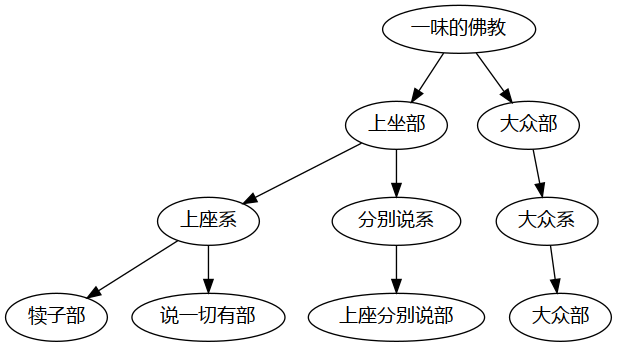
\includegraphics[scale=0.5]{释家/images/四派三系二部一味.png}


\chapter{名相}

\section{一}

\subsection{外道}
是佛典中的術語,梵語叫作底他迦(Tīrthaka),是指佛教以外之教道,或稱為外教、外學、外法。
凡是佛教以外的一切教道,以佛子視之,均為外道,初無輕藐之意;然以外教學者無不捨自己的身心而別求安頓,所以含有向外求道的意思者,即為外道。      

\section{二}

\section{三}

\subsection{三轉四諦}
\begin{itemize}
  \item 示轉:說明此是苦、此是集、此是滅、此是道。
  \item 勸轉:說明苦應知、集應斷、滅應證、道應修。
  \item 證轉:說明苦者我已知、集者我已斷、滅者我已證、道者我已修。
\end{itemize}

\subsection{三苦}
\begin{itemize}
  \item 苦苦
  \item 壞苦
  \item 行苦
\end{itemize}

\subsection{三連鎖}
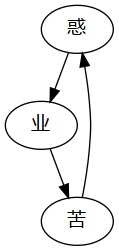
\includegraphics{释家/images/三连锁.png}
\begin{itemize}
  \item 惑:過去世的無明,現在世的愛及取。
  \item 業:過去世的行,現在世的有。
  \item 苦:現在世的識、名色、六入、觸、受,未來世的生及老死。
\end{itemize}

\section{四}

\subsection{四諦}
\begin{itemize}
  \item 苦諦:人生如苦海。
  \item 集諦:集是苦的原因,由煩惱而造業,由造業而招感苦的果報。
  \item 滅諦:滅是解脫苦果的可能,明瞭集諦之理,斷除煩惱之業,即可解脫眾苦。
  \item 道諦:道是滅苦的方法,修持八正道,即可滅除眾苦而獲涅槃解脫之果。
\end{itemize}

\subsection{四念住}
主要對治執身為凈、執受為樂、執心為常、執法為我的“四顛倒見”。
\begin{itemize}
  \item 身念住,觀身不凈
  \item 受念住,觀受是苦
  \item 心念住,觀心無常
  \item 法念住,觀法無我
\end{itemize}

\subsection{四正勤}
精進的重點在於行善去惡。
\begin{itemize}
  \item 未生惡法令不生;
  \item 已生惡法恒令滅;
  \item 未生善法令出生;
  \item 已生善法令增長。
\end{itemize}


\subsection{四神足}
意為產生精進的基礎
\begin{itemize}
  \item 欲神足,欲得見道;
  \item 勤神足,精勤習禪;
  \item 心神足,心神專一;
  \item 觀神足,正確觀想。
\end{itemize}

\section{五}

\subsection{五根}
修習佛法的根本所在。
\begin{itemize}
  \item 信根,深信三寶;
  \item 进根,修行不懈,指“四正勤”;
  \item 念根,憶念正法,指“四念處”;
  \item 定根,修習禪定;
  \item 慧根,開發智慧。
\end{itemize}

\subsection{五力}
由五根產生的五種力量。
\begin{itemize}
  \item 信力,堅信真理;
  \item 进力,修四正勤的力量;
  \item 念力,破邪、念正的力量;
  \item 定力,置心一處的能力;
  \item 慧力,產生智慧的能力。
\end{itemize}

\section{六}

\subsection{六度}
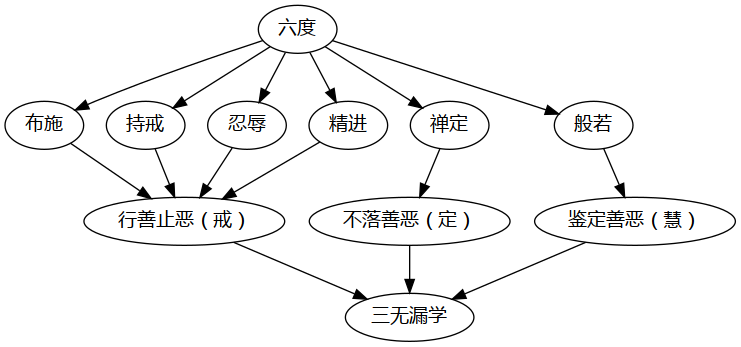
\includegraphics[scale=0.5]{释家/images/六度.png}
\begin{itemize}
  \item 布施
  \item 持戒
  \item 忍辱
  \item 精进
  \item 禅定
  \item 般若
\end{itemize}

\section{七}

\subsection{七众弟子}
順著次序等位來說;
通常所謂比丘二百五十戒,比丘尼五百戒,式叉摩尼六法,沙彌及沙彌尼十戒,優婆塞及優婆夷即是在家的男女弟子,有三皈五戒。
七眾的界別,即是根據所受持的戒法而定。
\begin{enumerate}
  \item 比丘(Bhikṣu)。
  \item 比丘尼(Bhikṣuṇī)\footnote{由於摩訶婆闍波提以及釋種五百女子的出家,便有了比丘尼。}。
  \item 式叉摩尼(Śāikṣamāṇā)。
  \item 沙彌(Śrāmaṇera)\footnote{由於少年羅睺羅的出家,僧中即有了沙彌。}。
  \item 沙彌尼(Śrāmaṇerikā)。
  \item 優婆塞(Upāsaka)\footnote{由於頻婆沙羅王的皈依佛教,在家的男女信徒即日漸增加}。
  \item 優婆夷(Upāsikā)。
\end{enumerate}


\subsection{七覺支}
修習止觀的注意事項和感受。
\begin{itemize}
  \item 念覺支,憶念集中而念念分明;
  \item 擇法覺支,選擇正確、適宜的修法;
  \item 精進覺支,任何階段都不能懈怠;
  \item 喜覺支,修禪定得到的喜悅;
  \item 輕安覺支,得到的輕鬆安適感覺;
  \item 定覺支,攝心不散深入禪定;
  \item 捨覺支,捨一切念,不即不離。
\end{itemize}

\subsection{七結(使)}
\begin{itemize}
  \item 欲貪
  \item 有貪
  \item 瞋恚
  \item 慢
  \item 見
  \item 疑
  \item 無明
\end{itemize}

\section{八}

\subsection{八苦}
苦苦之中又有八種
\begin{itemize}
  \item 生苦
  \item 老苦
  \item 病苦
  \item 死苦
  \item 愛別離苦
  \item 怨憎會苦
  \item 求不得苦
  \item 五蘊熾盛苦
\end{itemize}

\subsection{八正道}
八正道即是四聖諦中的道諦\footnote{由八正道,開演出三十七道品,又歸納演化為六波羅蜜多(六度),但其均屬於戒、定、慧的三無漏學的範圍。}
\begin{itemize}
  \item 正見:即是正確的見解。\footnote{何為正見?則應以三法印來鑑定}。
  \item 正思惟:即是以正見為基礎,而來思量熟慮此正見的內容,這是「意」業的實踐工夫。
  \item 正語:基於正確的意念,表達於「口」業的實踐工夫,不得對人妄言欺騙、綺語淫詞、兩舌挑撥、惡口罵辱,而且要做善言勸勉、愛語安慰。
  \item 正業:即是正當的身業,不做殺生、偷盜、淫亂、使用麻醉物等的惡業。配合意、語二業,即是「身、語、意」的三業清淨。
  \item 正命:即是正當的謀生方法,除了不做惡業,更應以正當職業,謀取生活所需。不得以江湖術數等的伎倆,騙取不義之財。
  \item 正精進:即是策勵自己,努力於道業。惡之尚有未斷者,立即求其斷,善之尚有未修者,立即求其修;未起之惡令不起,已修之善令增長。
  \item 正念:既已有了策勵精進之心,即應攝心制心,以不淨觀等方法,使心住於一境,不起物我之思。
  \item 正定:循著前面的七階段來修持,必可進入四禪八定,最後再以空慧之力,進入滅受想定,便是涅槃的解脫境界。
\end{itemize}

\section{九}

\subsection{九結}
以七結為基礎,但將有貪改為取,另加嫉、慳。
\begin{itemize}
  \item 欲貪
  \item 取
  \item 嫉
  \item 慳
  \item 瞋恚
  \item 慢
  \item 見
  \item 疑
  \item 無明
\end{itemize}

\section{十}

\subsection{《攝大乘論》十種殊勝相}
十種殊勝相可分為境、行、果的三類。一及二是境殊勝,三至八是行殊勝,九及十是果殊勝。
\begin{itemize}
  \item 所知依:「謂阿賴耶識,說名所知依體」。一切所應知的法,都依於阿賴耶識而立。也就是說,阿賴耶識為三性(遍計執、依他起、圓成實)所依。對三性有兩種見解:遍計執及依他起是雜染,圓成實是清淨。遍計執是雜染,圓成實是清淨,依他起通於雜染和清淨之二邊。照第一見解說,阿賴耶是虛妄不實、雜染不淨;照第二見解說,阿賴耶既是虛妄雜染,也是真實清淨。無著側重在第一種見解,世親則兼談兩種。
  \item 所知相:「三種自性」,「說名所知相體」。所知就是相,名為所知相。即是將一切所應知的法,分為三相來說明:1.依他起自性─是仗因托緣而生起的、可染可淨而不是一成不變的一切法。2.遍計所執自性─是指亂識(幻妄)所取的一切法,毫無實體,不過是一種自己的錯覺意境。3.圓成實自性─是指由人空及法空所顯的諸法之真實性。
  \item 入所知相:「唯識性,說名入所知相體」。由修唯識觀而悟入唯識性,就是悟入所知相的真實性。唯識觀有兩種:1.初步的方便唯識觀─以唯識觀觀一切法的自性為虛妄分別,所以了不可得。2.進一步的真實唯識觀─觀察諸法之境不可得,虛妄分別的識也不可得,心境俱泯,即悟入平等法性(圓成實性)。本論的唯識觀雖通於真實境(地上),但重於從凡入聖(由加行分別智到根本無分別智)的唯識觀。
  \item 彼入因果:「六波羅蜜多,說名彼入因果體」。彼入就是入彼,即是說,要悟入彼(那個)唯識的實性,必須修習六種波羅蜜多(布施、持戒、忍辱、精進、禪定、智慧);尚未悟入唯識性時,所修者是因,證入唯識性以後,所修者即是果。
  \item 彼因果修差別:「菩薩十地,說名彼因果修差別體」。進入初地以後的聖位菩薩,於十地中,仍是修習六波羅蜜多;地地增上,故說有十地差別。到佛果時,六波羅蜜多的修習,即告圓滿。
  \item 修差別中增上戒:「菩薩律儀,說名此中增上戒體」。即是諸地之中菩薩所修的戒學,表明他們不是修的聲聞小乘戒,故稱菩薩律儀。地地修習、展轉、增加、向上,故名增上。
  \item 增上心:「首楞伽摩,虛空藏等諸三摩地,說名此中增上心體」。此即是諸地菩薩所修的定學。定以心為主體,故稱增上心。首楞伽摩,義為健行,就是首楞嚴大定,此定境界很高,為十住菩薩所修。虛空藏也是定名,能含攝、能出生一切功德,所以名為虛空藏。
  \item 增上慧:「無分別智,說名此中增上慧體」。此即菩薩所修的慧學。無分別智含有加行智、根本智、後得智三者。菩薩遠離一切法執分別,故此三智皆稱無分別智。
  \item 彼果斷:「無住涅槃,說名彼果斷體」。彼果,就是修習那戒、定、慧三增上學所得的果。那果就是斷煩惱障及所知障而得的果,故稱果斷。無住涅槃是不住於生死也不離於生死之義。
  \item 彼果智:「三種佛身」,「說名彼果智體」。上面所說的那個果,就是智,故名果智。從果的斷障寂滅而言,是無住大般涅槃;從果顯現的智慧而言,是圓滿的無分別智,亦即是八識轉為四智而成就三種佛身:1.第八識轉成大圓鏡智、第七識轉成平等性智,即是「自性身」佛。2.第六識轉成妙觀察智,即是「受用身」佛。3.前五識轉為成所作智,即是「變化身」佛。第一種身是常住的,二、三種身是無常的。由自性身現起的受用身,受用一切法樂(自受用),並為地上的聖位菩薩說法(他受用);由自性身現起的變化身,則為聲聞說法。
\end{itemize}

\section{十二}

\subsection{十二因缘}
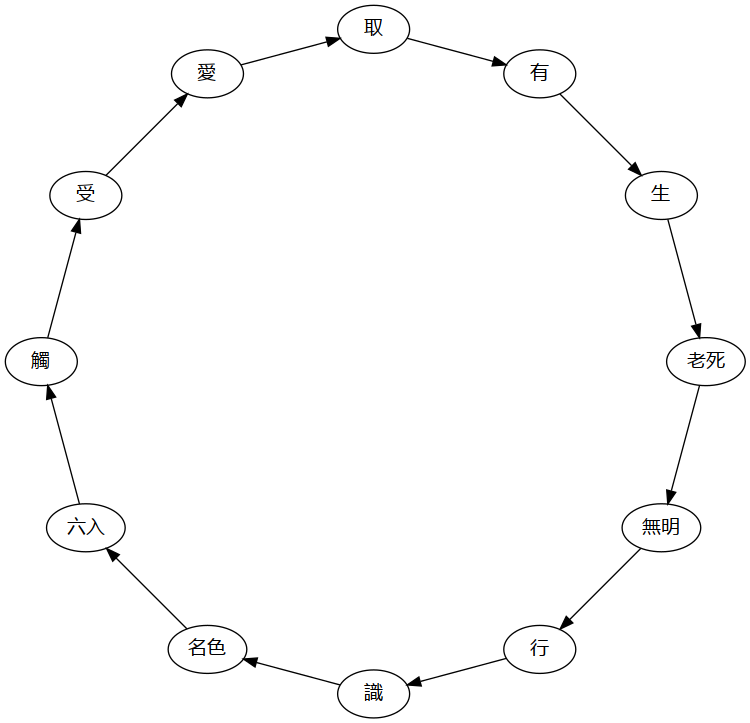
\includegraphics[scale=0.5]{释家/images/十二因缘.png}
苦、集二諦的解釋,是緣生法,也就是十二因緣\footnote{說明人生的由來和生命的流轉,自前生、今生而到後生之間的因果關係,即稱為三世兩重因果}法。
\begin{itemize}
  \item 無明:即是無智慧,是貪欲、瞋恨、愚癡等的煩惱,也是種種蠢動心理的迷惑之源。
  \item 行:即是前生造作的善惡諸業─身心的行為。
  \item 識:即是由過去世的業力,感受果報之初起妄念而托母胎,投為今生的神識。
  \item 名色:即是入胎後胎兒的身心狀態。
  \item 六入:即是在胎中長成的眼、耳、鼻、舌、身、意等六種感覺器官─六根。
  \item 觸:即是出胎後,自己的六根與外在的色、聲、香、味、觸、法等六塵相對接觸。
  \item 受:即是由接觸外境所感知的苦及樂的心境。
  \item 愛:即是厭苦欣樂而貪染財、色、名、食、睡等五欲的心理活動。
  \item 取:即是因欲愛旺盛而對於貪染諸境起取著心。
  \item 有:即是由於今生造作了有漏之因,而導致感受未來世的生死之果。
  \item 生:即是因了今生造作的業種,所感受來生的色、受、想、行、識的五蘊之身。
  \item 老死:來生既有了五蘊假合之身的出生,必將衰老而至死亡。
\end{itemize}
\begin{table}[H]
  \centering
  \small
  \caption[]{三世十二因缘}
  \begin{tabular}{|c|c|c|c|c|c|c|c|c|c|c|c|}
    \hline \multicolumn{2}{|c|}{未来世} & \multicolumn{8}{|c|}{现在世} & \multicolumn{2}{|c|}{过去世} \\
    \hline 老死 & 生 & 有 & 取 & 爱 & 受 & 触 & 六入 & 名色 & 识 & 行 & 无明 \\
    \hline \multicolumn{2}{|c|}{苦} & 业 & \multicolumn{2}{|c|}{惑} & \multicolumn{5}{|c|}{苦} & 业 & 惑 \\
    \hline \multicolumn{2}{|c|}{未来世的二果(苦谛)} & \multicolumn{3}{|c|}{现在世的三因(集谛)} & \multicolumn{5}{|c|}{现在世的五果(苦谛)} & \multicolumn{2}{|c|}{过去世的二因(集谛)} \\
    \hline \multicolumn{5}{|c|}{现在未来一重因果} & \multicolumn{7}{|c|}{过去现在一重因果} \\
    \hline \multicolumn{12}{|c|}{三世两重因果} \\
    \hline
  \end{tabular}
\end{table}

\section{十六}

\section{十八}


\chapter{高僧大德}
\section{佛陀十大弟子}

\subsection{須菩提}
譯作空生或善現 解空第一者,是證得無諍三昧者 般若經》多半由他為法 會的當機者。

\section{印顺导师}

\subsection{妙雲集}
\subsubsection{上編}
經論的解說
\begin{itemize}
  \item 《般若經講記》\footnote{這包含了《金剛經》及《心經》的兩部講記}
  \item 《寶積經講記》
  \item 《勝鬘經講記》
  \item 《藥師經講記》
  \item 《中觀論頌講記》
  \item 《攝大乘論講記》
  \item 《大乘起信論講記》
\end{itemize}
\subsubsection{中編}
是專著而篇幅超過十萬字的
\begin{itemize}
  \item 《佛法概論》
  \item 《中觀今論》
  \item 《唯識學探源》
  \item 《性空學探源》
  \item 《成佛之道》
  \item 《太虛大師年譜》
\end{itemize}
\subsubsection{下編}
是短篇的總集,不問是寫的,記錄的,都編在一起。
\begin{itemize}
  \item 《佛在人間》\footnote{重於人間佛教的現實利益,從人乘正行而向佛道。}
  \item 《學佛三要》\footnote{信願、智慧、慈悲——為大乘佛法的三要,學者要不偏不離的去學習。}
  \item 《以佛法研究佛法》
  \item 《淨土與禪》
  \item 《青年的佛教》
  \item 《我之宗教觀》
  \item 《無諍之辯》
  \item 《教制教典與教學》
  \item 《佛教史地考論》
  \item 《華雨香雲》
  \item 《佛法是救世之光》
\end{itemize}


\chapter{典故}
\section{佛陀十大弟子}


\chapter{《法鼓全集》}

\chapter{《妙云集》}

\chapter{《大正藏》}

\chapter{参考书籍}
\begin{itemize}
  \item 圣严法师$\cdot$《法鼓全集》
  \item 印顺法师$\cdot$《妙云集》
  \item 太虚大师$\cdot$《太虚大师全集》
\end{itemize}


  \printindex
\end{document}
